%File: formatting-instruction.tex
\documentclass[letterpaper]{article}
\usepackage{times}
\usepackage{helvet}
\usepackage{courier}
\usepackage{amssymb, amsmath, amsthm}
\usepackage{graphicx}
\usepackage{multirow}

\begin{document}

\subsection{Comparing Aggregate Statistics of Community Structure}

We begin by examining the overall statistics for the communities inferred by OSLOM using the weightings defined in Sections \ref{method-activity}, \ref{method-interaction}, and \ref{method-topic}. The number of communities by community type is given in Table~\ref{Table-comm_count}. We see that the topic- and interaction-based networks admit the most communities. The activity-based network admits the least number of communities.  One advantage of the OSLOM over many other community detection algorithms is that it explicitly accounts for singleton `communities': those nodes who do not belong to \emph{any} extant communities. This is especially important when a network is collected via a breadth-first search, as in our network, where we begin from a seed node and then branch out. Such a search, once terminated, will result in a collection of nodes on the periphery of the network that may not belong to any community in the core.

% See here
% 	http://arxiv.org/pdf/1202.2684v2.pdf
% for possible useful references on core-periphery networks.

The number of singletons by community type is also shown in Table~\ref{Table-comm_count}. We see that the topic- and interaction-based communities have the most singletons, with the activity-based community dominating this measure. This result for the activity-based community is an artifact of a property of the retweet/mention weighting: many of the users in the data set (\textbf{TK: give actual number}) did not interact with each other, and thus all of their edges were zero-weighted, leading to trivial singletons.

\begin{table}[ht]
	\label{Table-comm_count}
	\caption{Number of non-singleton communities and singletons by community type: S(tructural), A(ctivity -based), T(opic-based), and I(nteraction-based).}
	\centering
	\begin{tabular}{| c | c | c |}
		\hline Community Type & \# of Communities & \# of Singletons \\ \hline
		% Structural & 201 \\
		% Activity, Lag 1 & 101 \\
		% Activity, Lag 2 & 99 \\
		% Activity, Lag 3 & 106 \\
		% Activity, Lag 4 & 105 \\
		% Activity, Lag 5 & 107 \\
		% Activity, Lag 6 & 106 \\
		% Topic & 289 \\
		% Interaction & 252 \\ \hline
		S & 201 & 308 \\
		A, Lag 1 & 101 & 951 \\
		A, Lag 2 & 99 & 600 \\
		A, Lag 3 & 106 & 611 \\
		A, Lag 4 & 105 & 668 \\
		A, Lag 5 & 107 & 632 \\
		A, Lag 6 & 106 & 642 \\
		T & 289 & 1064 \\
		I & 252 & 2436 \\ \hline
	\end{tabular}
\end{table}

Next we consider the distribution of community sizes across the community types. The complementary cumulative distribution of community sizes is given in Figure~\ref{Fig-community_size_distribution}. Note that the axes are plotted on log-scale, and the horizontal axis begins with non-singleton communities. Thus, for a fixed community size $c$, Figure~\ref{Fig-community_size_distribution} shows the proportion of communities of size greater than $c$ for each community type. The largest communities for the structural, activity-based, topic-based, and interaction-based networks are 198, 358, 338, and 811 respectively.

\begin{figure}[ht]
  \centering
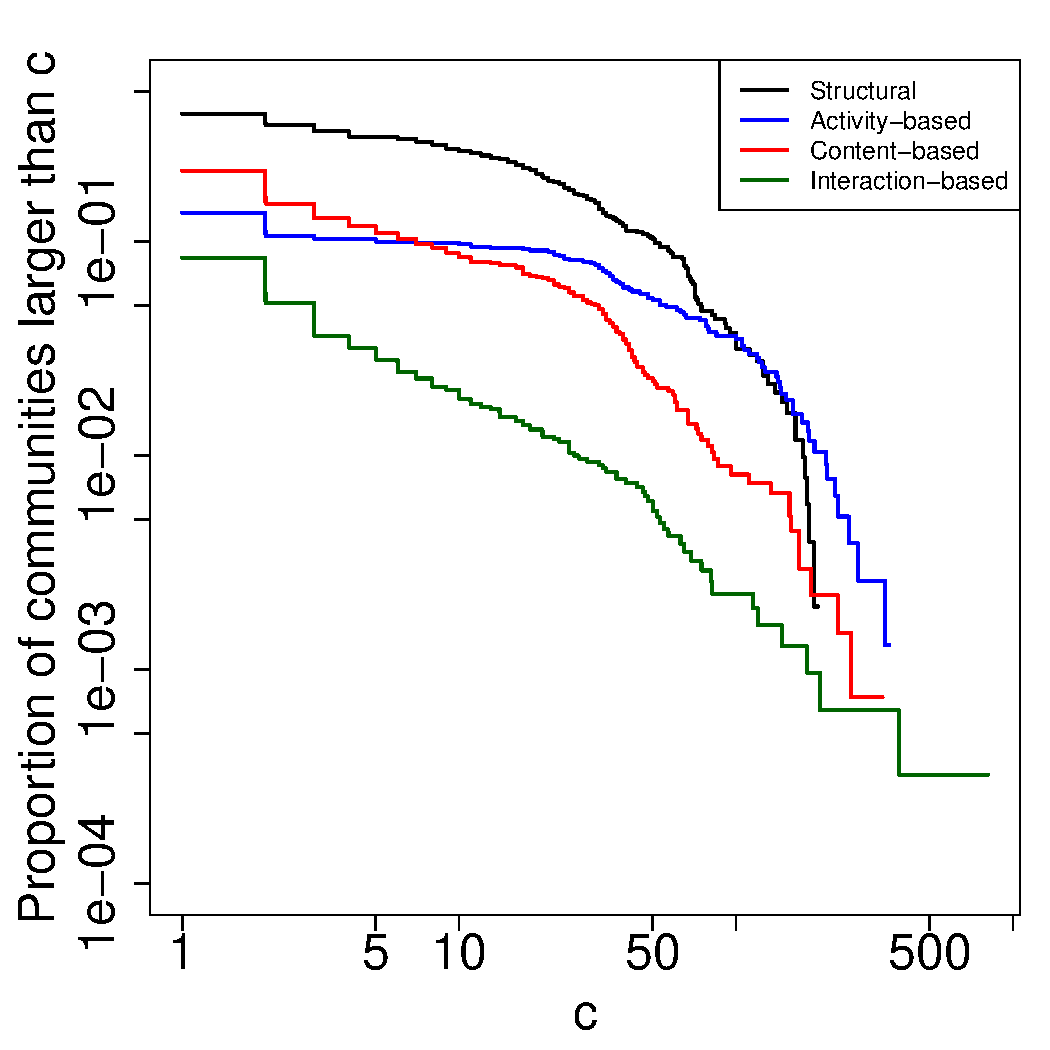
\includegraphics[width=0.50\textwidth]{../Figures/comm_sizes_ecdf_loglog.pdf}
\caption{The proportion of communities greater than $c$ in size, across the different community types. Note the logarithmic scale on the horizontal and vertical axes.}
\label{Fig-community_size_distribution}
\end{figure}

Next, we compare the number of users which belong to more than one community. Figure~\ref{Fig-overlap_plot} shows the number of users belonging to 2, 3, or 4 communities. We see that as the number of mixed membership communities increases, the number of users with that number of mixed memberships decreases. This is especially true for the activity-based community \textbf{TK: speculate on what this means? Or save for the results section?}.  In addition, \textbf{TK: mention the 5, 6, and 7 cases, not included in the figure}. This corresponded to \textbf{TK: investigate which users are the high-overlap and what communities they belong to.}

% The user with a structural overlap of 7 communities was 1630261,
%	https://twitter.com/marksilva

\begin{figure}[ht]
  \centering
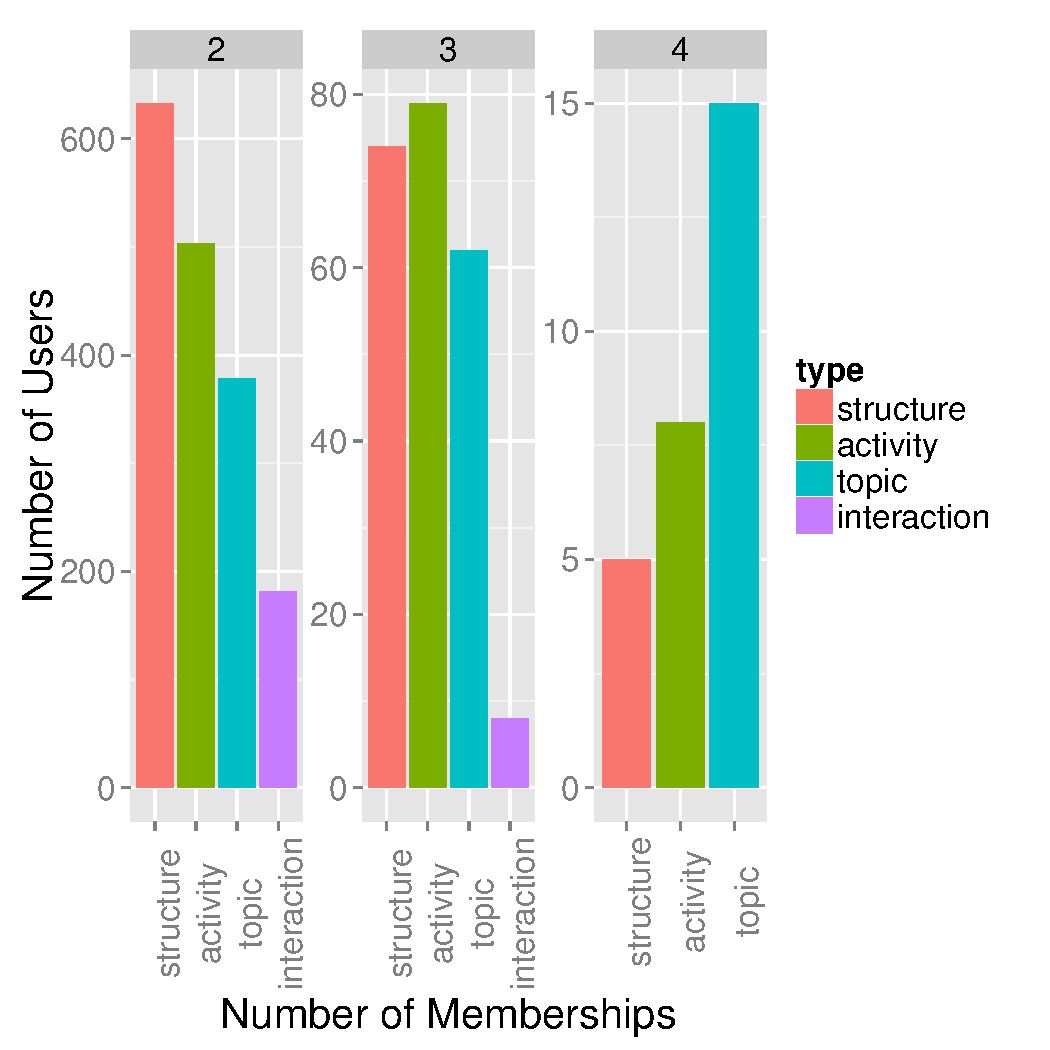
\includegraphics[width=0.50\textwidth]{../Figures/overlap_by_type.pdf}
\caption{The number of users belonging to 2, 3, or 4 communities, by community type.}
\label{Fig-overlap_plot}
\end{figure}

\end{document}